\section{Abstract Classes}

We consider a class to be abstract if it is not representable by any instance. That is, we cannot create an instance of an abstract class. Abstract classes are useful when we want to define a class that is a generalization of other classes, but we do not want to create instances of the generalization.

\example{Consider, once again, a hierarchy of animals.} There is no such thing as an ``animal'' or something that is solely called an animal. On the other hand, everything that we would categorize as an animal \emph{is} an animal. Therefore it makes sense to say that animals are a generalization of other types of ``sub''-animals. Imagine we want to write an \ttt{Animal} class, where we will say that any animal can speak. The abstract class contains a superfluous constructor as well as an abstract \ttt{speak} method. We define \ttt{speak} as abstract to denote that an animal can speak, but it is nonsensical for \ttt{Animal} to speak. Because it is impossible to instantiate an instance of \ttt{Animal}, it is similarly impossible to reasonably define \ttt{speak}.

\begin{cl}[]{Animal Class}
\begin{lstlisting}[language=MyJava]
abstract class Animal {

  Animal() {} 

  abstract String speak();
}
\end{lstlisting}
\end{cl}

Let's declare two subclasses: \ttt{Dog} and \ttt{Cat}, representing dogs and cats respectively. A cat can meow via the string \ttt{"Meow!"}, whereas a dog woofs via the string \ttt{"Woof!"}. 

\begin{cl}[]{Dog Class}
\begin{lstlisting}[language=MyJava]
class Dog extends Animal {

  Dog() { super(); }

  @Override
  String speak() { return "Woof!"; }
}
\end{lstlisting}
\end{cl}

\begin{cl}[]{Cat Class}
\begin{lstlisting}[language=MyJava]
class Cat extends Animal {

  Cat() { super(); }

  @Override
  String speak() { return "Meow!"; }
}
\end{lstlisting}
\end{cl}

It might seem strange to use an abstract class, since we could write a \ttt{Speakable} interface to do the same logic. The differences between abstract classes and interfaces is a blurry line to beginning Java programmers (and even to some who have been programming for years), but in essence, we use abstract classes when we want to enforce a class hierarchy of ``is-a'' relationships, e.g., a \ttt{Cat} is-a \ttt{Animal}, and a \ttt{Dog} is-a \ttt{Animal}. Moreover, abstract classes can contain non-abstract methods, meaning that a subclass needs not to override such methods. Interfaces, on the other hand, contain only methods that the implementing class must override. In addition to the method distinction, abstract classes may contain instance variables, whereas interfaces may not.\footnote{Both abstract classes and interfaces can contain static methods and variables.}

\example{Suppose we're writing a two-dimensional game that has different types of interactable objects in the world. The core game object stores the $(x, y)$ location, with nothing more. Again, we want to design a class that specific types of game objects can extend. For instance, our game might contain circular and rectangular objects. Of course, circles and rectangles have different dimension units, namely radius versus width and height respectively. We plan for each object to be interactable with one another. Unfortunately, collision detection is a complicated set of algorithms whose discussion far exceeds the scope of this text. Conversely, there is an extremely straightforward solution that involves treating all objects as rectangles. We call this technique \emph{axis-aligned bounding box}. Because not every object may be collidable, we will design a class \ttt{AxisAlignedBoundingBoxObject} that separately stores the object width and height as the dimensions of the bounding box. This class defines a method for colliding with another \ttt{AxisAlignedBoundingBoxObject}, which determines whether some point of $o_1$ is inside the bounding box of the $o_2$ object. This logic is not the focal point of the discussion, so we will only illustrate the example via an image and not explain the code itself. The purpose for this example is to demonstrate object hierarchy; not recreate the next best-selling two-dimensional side-scroller.}

\begin{figure}[H]
\centering
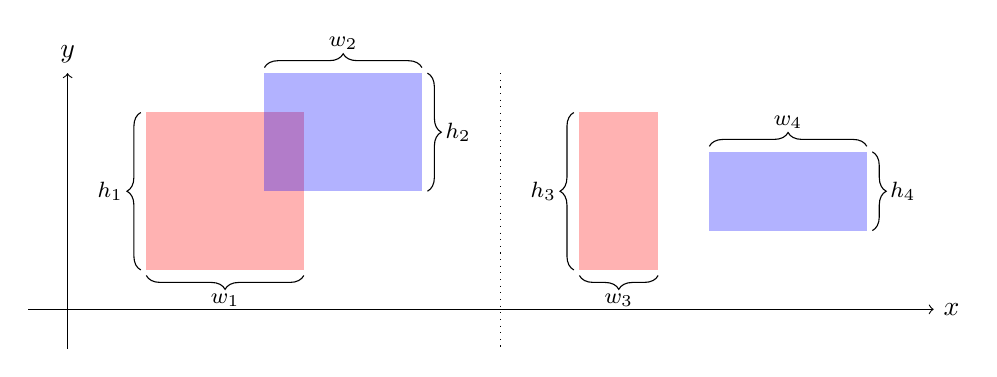
\begin{tikzpicture}[scale=1]

% Coordinates of Rectangle 1
\coordinate (A) at (1, .5);
\coordinate (B) at (3, .5);
\coordinate (C) at (3, 2.5);
\coordinate (D) at (1, 2.5);

% Coordinates of Rectangle 2
\coordinate (E) at (2.5, 1.5);
\coordinate (F) at (4.5, 1.5);
\coordinate (G) at (4.5, 3);
\coordinate (H) at (2.5, 3);

% Draw x/y axis
\draw[->] (-.5,0) -- (11,0) node[right] {\textbf{$x$}};
\draw[->] (0,-.5) -- (0,3) node[above] {\textbf{$y$}};
\draw[dotted] (5.5, 3) -- (5.5,-.5) node[above] {};

% Draw Rectangle 1 in transparent red
\fill[red, opacity=0.3] (A) -- (B) -- (C) -- (D) -- cycle;

% Draw Rectangle 2 in transparent blue
\fill[blue, opacity=0.3] (E) -- (F) -- (G) -- (H) -- cycle;

% Width labels for Rectangle 1
\draw[decorate, decoration={brace, amplitude=5pt, mirror, raise=2pt}] (A) -- (B) node[midway, below=5pt] {\footnotesize{}$w_1$};
\draw[decorate, decoration={brace, amplitude=5pt, raise=2pt}] (A) -- (D) node[midway, left=5pt] {\footnotesize{}$h_1$};

% Width labels for Rectangle 2
\draw[decorate, decoration={brace, amplitude=5pt, raise=2pt, mirror}] (G) -- (H) node[midway, above=5pt] {\footnotesize{}$w_2$};
\draw[decorate, decoration={brace, amplitude=5pt, raise=2pt, mirror}] (F) -- (G) node[midway, right=5pt] {\footnotesize{}$h_2$};

% Coordinates of Rectangle 3
\coordinate (I) at (6.5, .5);
\coordinate (J) at (7.5, .5);
\coordinate (K) at (7.5, 2.5);
\coordinate (L) at (6.5, 2.5);

% Coordinates of Rectangle 4
\coordinate (M) at (8.15, 1);
\coordinate (N) at (10.15, 1);
\coordinate (O) at (10.15, 2);
\coordinate (P) at (8.15, 2);

% Draw Rectangle 3 in transparent red
\fill[red, opacity=0.3] (I) -- (J) -- (K) -- (L) -- cycle;

% Draw Rectangle 4 in transparent blue
\fill[blue, opacity=0.3] (M) -- (N) -- (O) -- (P) -- cycle;

% Width labels for Rectangle 3
\draw[decorate, decoration={brace, amplitude=5pt, mirror, raise=2pt}] (I) -- (J) node[midway, below=5pt] {\footnotesize{}$w_3$};
\draw[decorate, decoration={brace, amplitude=5pt, raise=2pt}] (I) -- (L) node[midway, left=5pt] {\footnotesize{}$h_3$};

% Width labels for Rectangle 4
\draw[decorate, decoration={brace, amplitude=5pt, raise=2pt, mirror}] (O) -- (P) node[midway, above=5pt] {\footnotesize{}$w_4$};
\draw[decorate, decoration={brace, amplitude=5pt, raise=2pt, mirror}] (N) -- (O) node[midway, right=5pt] {\footnotesize{}$h_4$};
\end{tikzpicture}
\caption{Collision Detection Between Rectangles.}
\label{fig:collisiondetection}
\end{figure}

\begin{cl}[]{Game Object Class Definition}
\begin{lstlisting}[language=MyJava]
abstract class GameObject {
  
  private int x;
  private int y;

  GameObject(int x, int y) {
    this.x = x;
    this.y = y;
  }

  // Getters and setters omitted.
}
\end{lstlisting}
\end{cl}

\begin{cl}[]{Axis-Aligned Bounding Box Class}
\begin{lstlisting}[language=Myjava]
abstract class AxisAlignedBoundingBoxObject extends GameObject {
  
  private int width;
  private int height;

  AxisAlignedBoundingBoxObject(int x, int y, int width, int height) {
    super(x, y);
    this.width = width;
    this.height = height;
  }

  /**
   * Determines whether this object collides with another AxisAlignedBoundingBoxObject.
   * @param obj - instance of AxisAlignedBoundingBoxObject.
   * @return true if the objects overlap and false otherwise.
   */
  boolean collidesWith(AxisAlignedBoundingBoxObject obj) {
    return (this.getX() < obj.getX() + obj.width) &&
	   (this.getX() + this.width >= obj.getX()) &&
 	   (this.getY() < obj.getY() + obj.height)  &&
	   (this.getY() + this.height >= obj.height); 
  }
  
  // Getters and setters omitted.
}
\end{lstlisting}
\end{cl}

We declared an abstract class to extend another abstract class; which is perfectly acceptable. Because it makes no sense to have an entity called \ttt{AxisAlignedBoundingBoxObject}, we declare it as abstract, but we need it to contain the functionality of \ttt{GameObject}, which calls for the inheritance. Normally, we would immediately write an extensive test suite for \ttt{collidesWith}, but because we cannot instantiate an \ttt{AxisAlignedBoundingBox} directly, we cannot test \ttt{collidesWith} at the moment. In a couple of paragraphs, however, this will be possible, with the additions of \ttt{CircleObject} and \ttt{RectangleObject}.

\begin{cl}[]{Testing AABB Collision Detection}
\begin{lstlisting}[language=MyJava]
import static Assertions.assertAll;
import static Assertions.assertEquals;

class AxisAlignedBoundingBoxObjectTester {

  @Test
  void testCollidesWith() {
    AxisAlignedBoundingBoxObject o1 = new RectangleObject(30, 30, 1000, 2000);
    AxisAlignedBoundingBoxObject o2 = new RectangleObject(0, 0, 5, 5);
    AxisAlignedBoundingBoxObject o3 = new RectangleObject(400, 200, 750, 250);
    AxisAlignedBoundingBoxObject o4 = new RectangleObject(300, 100, 300, 200);
    AxisAlignedBoundingBoxObject o5 = new CircleObject(20, 30, 1000);
    AxisAlignedBoundingBoxObject o6 = new CircleObject(200, 250, 500);
    AxisAlignedBoundingBoxObject o7 = new CircleObject(30, 300, 1500);
    AxisAlignedBoundingBoxObject o8 = new CircleObject(90, 85, 200);
    assertAll(
      () -> assertTrue(o1.collidesWith(o2)),
      () -> assertTrue(o1.collidesWith(o4)),
      () -> assertTrue(o2.collidesWith(o3)),
      () -> assertTrue(o2.collidesWith(o8)),
      () -> assertTrue(o3.collidesWith(o5)),
      () -> assertTrue(o5.collidesWith(o4)),
      () -> assertTrue(o6.collidesWith(o7)),
      () -> assertTrue(o7.collidesWith(o3)));
  }
}
\end{lstlisting}
\end{cl}

We need to translate our circles into axis-aligned bounding box, but what does that mean? In short, we convert the given radius into the corresponding diameter, and designate this diameter as the width and height of the bounding box. Rectangular objects, on other hand, need no such fancy translation, since a bounding box is a rectangle. Neither subclasses storetheir dimensions as instance variables, due to the fact that the superclass takes care of this for us.

The question that we anticipate many readers are thinking of is, why do we even distinguish objects of differing ``types'' if they both implement collision detection in the same fashion? Since we are working in the context of a game, the way we draw these objects will almost certainly be different! Let's, for the sake of emphasizing the distinctions, design a \ttt{IDrawable} interface, which provides one method: \ttt{draw(Graphics2D g2d)}, which gives us a \ttt{Graphics2D} object. We will not discuss, nor do we really care about the innards of a graphics library aside from the fact that it contains two primitive methods: \ttt{drawOval(int x, int y, int w, int h)} and \ttt{drawRect(int x, int y, int w, int h)}. Therefore our two object subclasses will implement \ttt{IDrawable} and override the method differently.

\begin{cl}[]{Drawable Interface Definition}
\begin{lstlisting}[language=MyJava]
interface IDrawable {
  
  /**
   * Provides a means of drawing primitive graphics.
   * The inner details of "Graphics2D" are not important to us; 
   * we care about the fact that we can use the following methods:
   * 
   * - drawOval(int x, int y, int w, int h);
   * - drawRect(int x, int y, int w, int h);
   */
  void draw(Graphics2D g2d); 
}
\end{lstlisting}
\end{cl} 

\begin{cl}[]{Circle Object Class Definition}
\begin{lstlisting}[language=MyJava]
class CircleObject extends AxisAlignedBoundingBoxObject implements IDrawable {
  
  CircleObject(int x, int y, int r) { super(x, y, r * 2, r * 2); }

  @Override
  void draw(Graphics2D g2d) {
    g2d.drawOval(this.getX(), this.getY(), this.getWidth(), this.getHeight());
  }
}
\end{lstlisting}
\end{cl}

\begin{cl}[]{Rectangle Object Class Definition}
\begin{lstlisting}[language=MyJava]
class RectangleObject extends AxisAlignedBoundingBoxObject implements IDrawable {
  
  RectangleObject(int x, int y, int w, int h) { super(x, y, w, h); }
  
  @Override
  void draw(Graphics2D g2d) {
    g2d.drawRect(this.getX(), this.getY(), this.getWidth(), this.getHeight());
  }
}
\end{lstlisting}
\end{cl}

\example{A terminal argument parser is a program/function that interprets a series of arguments passed to another program and makes it easier for programmers to determine if a flag is enabled. Without one, many programmers often resort to using a complex series of conditional statements to check for the existence of a flag. Not only is this cumbersome, but it is prone to errors, and neither extendable nor flexible to different arrangements of arguments. In this example we will develop a small terminal argument parser.}

First, we need to design a class that represents an ``argument'' to a program. Arguments, as we described in Chapter~\ref{chapter-arrays-collections}, are space-separated string values that we pass to a program executable, which populate the \ttt{String[] args} array in the \ttt{main} method. In particular, however, we want to specify that an argument is not necessarily the values themselves, but are instead the flags, or instructions, passed to the executable. The simplest version of a flag is one that receives exactly one argument, which we will represent via an abstract \ttt{Argument} class. Later on, we want to be able to validate a flag with its given arguments, so the \ttt{Argument} class includes an abstract \ttt{boolean validate} method, that shall be overridden in all subclasses of \ttt{Argument}.

\begin{cl}[]{Argument Class Definition}
\begin{lstlisting}[language=MyJava]
import java.util.List;
import java.util.Map;

abstract class Argument {

  private String key;

  Argument(String key) { this.key = key; }

  String getKey() { return this.key; }

  abstract boolean validate(Map<String, List<String>> args);
}
\end{lstlisting}
\end{cl}

From here, let's design two types of arguments: one that is optional and one that receives $n$ arguments. Namely, an optional argument is one that is always valid, according to \ttt{validate}, because it does not necessarily need to exist. The $n$-valued argument, on the other hand, requires that the associated passed flag contains exactly $n$ values. For example, if we say that the \ttt{--input} flag requires exactly $3$ arguments, then if we do not pass exactly three space-separated non-flag values, it fails to validate.

\begin{cl}[]{Optional Argument Implementation}
\begin{lstlisting}[language=MyJava]
import java.util.List;
import java.util.Map;

class OptionalArgument extends Argument {

  OptionalArgument(String key) { super(key); }

  @Override
  boolean validate(Map<String, List<String>> args) { return true; }
}
\end{lstlisting}
\end{cl}

\begin{cl}[]{Numbered Argument Implementation}
\begin{lstlisting}[language=MyJava]
import java.util.List;
import java.util.Map;

class NumberedArgument extends Argument {

  private final int NUM_REQUIRED_ARGS;

  NumberedArgument(String key, int n) {
    super(key);
    this.NUM_REQUIRED_ARGS = n;
  }

  @Override
  boolean validate(Map<String, List<String>> args) {
    if (!args.containsKey(this.getKey())) { return false; } 
    else { return args.get(this.getKey()).size() == this.NUM_REQUIRED_ARGS; }
  }
}
\end{lstlisting}
\end{cl}

Now comes the argument parser itself, which receives a string array of argument values, much like \ttt{main}, and extracts out the flags and arguments into a \ttt{Map<String, List<String$>$$>$} where the key represents the flag and the value is a list of the arguments to said flag. We also store a \ttt{Set<Argument>} to allow the programmer to designate arguments to the parser. The idea is straightforward: while traversing over \ttt{args}, if we encounter a string that begins with a double dash `\ttt{--}', it is qualified as a flag and the following arguments, up to another flag, are marked as arguments to the flag. We add these to the respective map as described before, and continue until we run out of elements in the array.

\begin{cl}[]{Terminal Arguments Parser Implementation}
\begin{lstlisting}[language=MyJava]
import java.util.Map;
import java.util.HashMap;
import java.util.Set;
import java.util.HashSet;

class ArgumentParser {

  private Map<String, List<String>> parsedArguments;
  private Set<Argument> arguments;

  ArgumentParser(String[] args) {
    this.arguments = new HashSet<>();
    this.parsedArguments = new HashMap<>();
    String currKey = null;
    for (String arg : args) {
      if (arg.startsWith("--")) {
        currKey = arg.split("--")[1];
        this.parsedArguments.putIfAbsent(currKey, new ArrayList<>());
      } else if (currKey != null) {
        this.parsedArguments.get(currKey).add(arg);
      }
    }
  }

  void addArgument(Argument arg) { this.arguments.add(arg); }

  List<String> getArguments(String key) {
    return this.parsedArguments.containsKey(key) ? 
             this.parsedArguments.get(key) : 
             null;
  }
}
\end{lstlisting}
\end{cl}

The \ttt{parseArguments} method returns whether or not the supplied arguments are valid according to the arguments populated via \ttt{addArgument}. Using streams, we verify that, after invoking \ttt{validate} on every argument, each separate call returns true, meaning that all arguments are valid and correct. Because it might be useful to return the associated arguments to a flag from a programmer's perspective who uses this parser, we include a \ttt{getArguments} method to return the list of arguments passed to a flag.

\begin{cl}[]{Tester for Terminal Arguments Parser}
\begin{lstlisting}[language=MyJava]
import java.util.Map;
import java.util.HashMap;
import java.util.Set;
import java.util.HashSet;

class ArgumentParser {
  
  // ... other methods not shown.

  /**
   * Determines whether or not all of the arguments in the stored
   * instance variable are "valid".
   * @return true if all arguments are valid, false otherwise.
   */
  boolean parseArguments() {
    return this.arguments.stream()
                         .allMatch(e -> e.validate(this.parsedArguments));
  }
}
\end{lstlisting}
\end{cl}

\example{Inheritance is a truly powerful programming language construct, and we will now attempt to describe its beauty through the design of a mini-project. Said mini-project will encompass writing a small programming language. Programming language syntax and semantics, collectively, require a lot of knowledge outside the domain and scope of this text, but we will see that, even with our somewhat limited arsenal of tools, we can construct a fairly powerful programming language. Our language will start off as a recreation of the interpreter from our section on interfaces, but contains modifications to make it more flexible.}

Programming language syntax is often broken up into the nodes of an \emph{abstract syntax tree}, which at a quick glance is nothing more than a description of the operations of a language. To begin, we need to describe our programming language capabilities. To keep things simple, our language will contain integers, variables, a few arithmetic operators, and conditionals. It's important to note that, because we are glossing over the innards of lexing and  parsing, all of our tests will exist in the form of abstract syntax trees. We want an abstract AST node class from which every other AST node inherits. Then, we can design purpose-specific nodes that do what we wish. Every abstract syntax tree has a list of children node. We will also define a \texttt{toString} method that will print out the abstract syntax tree in a readable format. Our abstract syntax tree class uses two constructors: one that receives a list of abstract syntax tree nodes, and another that is variadic over the \ttt{AstNode} type. We implement two different constructors for convenience purposes during testing.

Additionally, we want our abstract syntax trees to be evaluable. Because ``evaluable'' describes a behavior of a class, we should throw this into an interface. We want its method, namely \ttt{eval}, to return something of type \ttt{Lvalue} and receive an environment. For the time being, since we do not know what either an \ttt{Lvalue} or an \ttt{Environment} is, we will omit the definition of the interface, but include the overridden method inside \ttt{AstNode}. Notice, however, that we mark \ttt{eval} as \ttt{abstract} inside \ttt{AstNode}, because it is definitionally impossible to evaluate an \ttt{AstNode}, since evaluation behavior is dependent on the subclasses and how they interact.

An \ttt{Lvalue} is the left-hand side of the evaluation of an abstract syntax tree. That is, it is the value that a node resolves to after evaluation. As an example, consider an abstract syntax tree that represents a conditional expression. After evaluating the tree, we expect the resulting value to be either the evaluated consequent or the alternative, neither of which are abstract syntax trees themselves. So, we will design a class that encapsulates an abstract syntax tree, and returns the underlying value when prompted. For our programming language, an abstract syntax tree can only resolve to a number or a boolean, since they are the most primitive forms. Because we may need to retrieve the abstract syntax tree of an l-value, we will provide the relevant accessor method. For simplicity, will compare l-values based on their abstract syntax tree string representations.

\begin{cl}[]{Abstract Syntax Tree Class}
\begin{lstlisting}[language=MyJava]
import java.util.List;

abstract class AstNode implements Evaluable {

  private final List<AstNode> CHILDREN;  
 
  AstNode(List<AstNode> children) { 
    this.CHILDREN = children; 
  }

  AstNode(AstNode... children) { 
    this(List.of(children)); 
  }

  @Override
  abstract Lvalue eval(Environment env);

  List<AstNode> getChildren() { 
    return this.CHILDREN; 
  }

  public abstract String toString();
}
\end{lstlisting}
\end{cl}

\begin{cl}[]{L-value Class}
\begin{lstlisting}[language=MyJava]
final class Lvalue {

  private final AstNode VALUE;

  Lvalue(AstNode value) { 
    this.VALUE = value; 
  }

  AstNode getAst() { 
    return this.VALUE; 
  }

  double getNumValue() { 
    return ((NumberNode) this.VALUE).getValue(); 
  }

  boolean getBoolValue() { 
    return ((BoolNode) this.VALUE).getValue(); 
  }

  @Override
  public boolean equals(Object o) {
    if (o instanceof Lvalue) { 
      return this.toString().equals(o.toString()); 
    } else { 
      return false; 
    }
  }
}
\end{lstlisting}
\end{cl}

From here, the simplest three abstract syntax tree nodes are \ttt{VarNode}, \ttt{NumberNode}, and \ttt{BoolNode}, corresponding to variables, numbers, and booleans, respectively. Each of these nodes will have a single value, that being the variable name, number, or boolean. The \ttt{eval} methods of the latter two classes return an l-value that wraps themselves, since these values resolve to themselves. The former, that being \ttt{VarNode}, is a little trickier. We must consider what happens when we evaluate a variable in any other programming language. The language looks up the variable identifier in the list of accessible bindings and returns whatever is the corresponding value. This location of bindings is called an environment in the programming languages nomenclature, and generally takes the form of a \ttt{HashMap} data structure. Therefore we can store an instance of a \ttt{HashMap} in our \ttt{Environment} class. The question now is of what type are the keys and values in our map. Fortunately this is simple to determine; the keys are string identifiers, and the values are their corresponding abstract syntax trees. Our environment representation/class is extremely simple and almost seems superfluous, but in due time we will add more functionality to justify its existence over a simple \ttt{HashMap} instance.

\begin{cl}[]{Environment Class Implementation}
\begin{lstlisting}[language=MyJava]
import java.util.HashMap;
import java.util.Map;

final class Environment {
  
  private final Map<String, AstNode> ENV;

  Environment() { 
    this.ENV = new HashMap<>(); 
  }
}
\end{lstlisting}
\end{cl}

\begin{cl}[]{Testing Abstract Syntax Tree Tests}
\begin{lstlisting}[language=MyJava]
import static Assertions.assertEquals;
import static Assertions.assertAll;

class AstTest {

  @Test
  void testVarNode() {
    assertEquals("x", new VarNode("x").toString());
  }

  @Test
  void testNumberNode() {
    assertEquals("42", new NumberNode("42").toString());
  }

  @Test
  void testBoolNode() {
    assertEquals("true", new BoolNode("true").toString());
    assertEquals("false", new BoolNode("false").toString());
  }  
}
\end{lstlisting}
\end{cl}

\begin{cl}[]{Variable Node}
\begin{lstlisting}[language=MyJava]
final class VarNode extends AstNode {

  private final String NAME;

  VarNode(String name) {
    super();
    this.NAME = name;
  }

  /**
  * Interpret a variable. We look up the variable in the environment and
  * return the value associated with it.
  * @param env - the environment in which to interpret the variable.
  * @return The result of the variable lookup after interpretation.
  */
  @Override
  Lvalue eval(Environment env) {
    String id = this.NAME;
    AstNode res = env.get(id);
    return res.eval(env);
  }

  @Override
  public String toString() { 
    return this.NAME; 
  }
}
\end{lstlisting}
\end{cl}

\begin{cl}[]{Number Node}
\begin{lstlisting}[language=MyJava]
final class NumberNode extends AstNode {

  private final double VALUE;

  NumberNode(String value) {
    super();
    this.VALUE = Double.parseDouble(value);
  }

  NumberNode(double value) { 
    this(Double.toString(value)); 
  }

  @Override
  Lvalue eval(Environment env) { 
    return new Lvalue(this); 
  }

  @Override
  public String toString() { 
    return Double.toString(this.VALUE); 
  }
}
\end{lstlisting}
\end{cl}

\begin{cl}[]{Boolean Node}
\begin{lstlisting}[language=MyJava]
final class BoolNode extends AstNode {

  private final boolean VALUE;

  BoolNode(String value) {
    super();
    this.VALUE = Boolean.parseBoolean(value);
  }

  BoolNode(boolean value) { this(Boolean.toString(value)); }

  @Override
  Lvalue eval(Environment env) { return new Lvalue(this); }

  @Override
  public String toString() { return Boolean.toString(this.VALUE); }
}
\end{lstlisting}
\end{cl}

From here, we arrive at primitive operators via \ttt{PrimNode}. A primitive operator is one akin to addition, subtraction, and so forth. Two additional primitives that we will support are reading an integer from standard input, and printing one to standard output. Primitive operators receive any number of arguments and whose behavior is handled as a case analysis of the \ttt{eval} method. 

\begin{cl}[]{Primitive Operator Node}
\begin{lstlisting}[language=MyJava]
final class PrimNode extends AstNode {

  private final String OP;

  PrimNode(String op, AstNode... children) {
    super(children);
    this.OP = op;
  }

  /**
   * Interpret a primitive operation.
   * @param env - the environment in which to interpret the operation.
   * @return The result of the primitive operation.
   */
  @Override
  Lvalue eval(Environment env) {
    String op = this.OP;
    List<Lvalue> operands = this.getChildren().stream()
                                              .map(n -> n.eval(env))
                                              .toList();
    switch (op) {
      case "+": return this.primPlus(operand, env);
      case "-": return this.primMinus(operand, env);
      case "*": return this.primProduct(operand, env);
      case "eq?": return this.primEq(operand, env);
      default: return null;
    }
  }

  @Override
  public String toString() {
    return String.format("(%s %s)", this.OP, this.getChildren().toString());
  }
}
\end{lstlisting}
\end{cl}

\begin{cl}[]{Addition Primitive Operator}
\begin{lstlisting}[language=MyJava]
final class PrimNode extends AstNode {

  /**
   *
   * @param args - 
   * @param env - 
   * @return 
   */
  private Lvalue primPlus(List<Lvalue> args, Environment env) {
    return new Lvalue(args.stream().map(Lvalue::getNumValue).reduce(0.0, Double::sum));
  }
}
\end{lstlisting}
\end{cl}

\begin{cl}[]{Subtraction Primitive Operator}
\begin{lstlisting}[language=MyJava]
final class PrimNode extends AstNode {

  /**
   *
   * @param args - 
   * @param env - 
   * @return 
   */
  private Lvalue primMinus(List<Lvalue> args, Environment env) {
    return new Lvalue(args.stream().map(Lvalue::getNumValue).reduce(0.0, (a, c) -> c - a));
  }
}
\end{lstlisting}
\end{cl}

\begin{cl}[]{Multiplication Primitive Operator}
\begin{lstlisting}[language=MyJava]
final class PrimNode extends AstNode {

  /**
   *
   * @param args - 
   * @param env - 
   * @return 
   */
  private Lvalue primProduct(List<Lvalue> args, Environment env) {
    return new Lvalue(args.stream().map(Lvalue::getNumValue).reduce(1.0, (a, c) -> c * a));
  }
}
\end{lstlisting}
\end{cl}

\begin{cl}[]{Equality Primitive Operator}
\begin{lstlisting}[language=MyJava]
final class PrimNode extends AstNode {

  /**
   *
   * @param args - 
   * @param env - 
   * @return 
   */
  private Lvalue primEq(List<Lvalue> args, Environment env) {
    return new Lvalue(args.get(0).equals(args.get(1)));
  }
}
\end{lstlisting}
\end{cl}

We need a way of binding variables, so we shall take a hint from functional programming languages via the \ttt{LetNode} class. The \ttt{LetNode} class has three children: a variable name, a value, and a body. The variable name will be a string, with the value and body both being abstract syntax tree nodes. The \ttt{LetNode} class will have a \ttt{toString} method that will return a string in the form of \ttt{(let ([<var> <exp>]) <body>)}. The \ttt{eval} method will evaluate the value, extend the environment with the new binding, and then evaluate the body with the extended environment. To do this, we need to understand what environment extension entails. Reconsidering our \ttt{Environment} class, we know that it contains a \ttt{HashMap} to designate that environments use maps by design. We may be tempted to write a \ttt{set} method in our \ttt{Environment} class to add an identifier binding to the current environment. Although this works (and will be a necessity in due time), it means that we can only \emph{modify}, or \emph{change}, the environment, which isn't desired. The alternative approach would be to utilize \emph{environment extension}. That is, create a new environment with the old bindings, followed by an insertion of the new binding. Environment extension brings up the issue of variable scope, because different variables are live at different locations in the program. Consider the following program described by the abstract syntax tree:

\begin{verbnobox}[\small]
new LetNode("x", new NumberNode(5), 
 new LetNode("y", new PrimNode("+", new NumberNode(6), new VarNode("x")), 
  new VarNode("y")))
\end{verbnobox}
  
Within the inner-most \ttt{PrimNode} expression, $x$ does not exist in its environment, but it does exist in an environment defined above its scope. So, each environment is itself a store a map of identifiers to abstract syntax trees, but they also contain another \ttt{Environment}. If we are at the ``root level'' of the program, this environment is set to \ttt{null}. Correspondingly, Environment contains two constructors: one that receives a parent environment and another without. As such, we must write the \ttt{lookup} method, which finds a variable binding in the current list of bindings and, if it does not exist, recursively looks it up in the parent environment. If we reach the root level environment and the variable does not exist, we return a \ttt{null} value. We also override the \ttt{toString} method to print out the environment in a readable format.

\begin{cl}[]{Environment Tester}
\begin{lstlisting}[language=MyJava]
import static Assertions.assertEquals;
import static Assertions.assertAll;

class EnvironmentTester {
  
  @Test
  void testEnvironment() {
    Environment root = new Environment();
    Environment e1 = env.extend("x", new NumberNode(5));
    Environment e2 = env.extend("y", new NumberNode(6));
    assertAll(
      () -> assertEquals(new NumberNode(5), env.lookup("x")),
      () -> assertEquals(new NumberNode(6), env.lookup("y")),
      () -> assertEquals(null, env.lookup("z")),
      () -> assertEquals(null, env.lookup("x")));
  }
}
\end{lstlisting}
\end{cl}
  
\begin{cl}[]{Environment Class}
\begin{lstlisting}[language=MyJava]
import java.util.HashMap;
import java.util.Map;

final class Environment {

  private final Map<String, AstNode> ENV;
  private final Environment PARENT;

  Environment() { 
    this(null); 
  }

  Environment(Environment parent) { 
    this.ENV = new HashMap<>(); 
    this.PARENT = parent; 
  }

  /**
   * Looks up a variable in the current environment.
   * @param id - the variable name.
   * @return the value bound to the variable, or null if it does not exist.
   */
  @Override
  AstNode lookup(String id) {
    if (this.ENV.containsKey(id)) { 
      return this.ENV.get(id); 
    } else if (this.PARENT != null) { 
      return this.PARENT.ENV.lookup(id); 
    } else { 
      return null; 
    }
  }

  /**
   * Extends the current environment to contain a new variable binding.
   * @param id - the variable name.
   * @param value - the value to bind to the variable.
   * @return a new environment with the new binding.
   */
  Environment extend(String id, AstNode value) {
    Environment env = new Environment(this);
    env.ENV.put(id, value);
    return env;
  }
}
\end{lstlisting}
\end{cl} 

Our modified version of the environment allows us to implement local/let bindings in a way that respects parent environments. As one of the exercises of this chapter demonstrate, environment extension helps us when adding user-defined functions.

\begin{cl}[]{Let Node}
\begin{lstlisting}[language=MyJava]
final class LetNode extends AstNode {

  private final String ID;

  LetNode(String id, AstNode exp, AstNode body) {
    super(exp, body);
    this.ID = id;
  }

  /**
   * Interpret a let statement. A new environment is introduced 
   * in which the let body is evaluated.
   * @param env - The environment in which to interpret the let binding.
   * @return The result of the let statement.
   */
  @Override
  Lvalue eval(Environment env) {
    String id = this.ID;
    AstNode exp = this.getChildren().get(0);
    AstNode body = return this.getChildren().get(1);

    // Interpret the expression and convert it into its AST.
    AstNode newExp = exp.eval(env).getAst();
    Environment e1 = env.extend(var, newExp);
    return body.eval(e1);
  }

  @Override
  public String toString() {
    AstNode e = this.getChildren().get(0);
    AstNode b = this.getChildren().get(1);
    return String.format("(let ([%s %s]) %s"), this.VAR, e.toString(), b.toString());
  }
}
\end{lstlisting}
\end{cl}

Finally we arrive at decision-based nodes. The \ttt{IfNode} class represents a conditional expression rather than a statement. Recall the ternary operator; it resolves to a value, unlike Java's \ttt{if} statement. The \ttt{IfNode} class has three children: a predicate, a consequent, and an alternative. The predicate is an abstract syntax tree that represents a boolean expression, and the consequent and alternative are arbitrary abstract syntax tree nodes. The \ttt{IfNode} class will have a \ttt{toString} method that will return a string of the form \ttt{(if <pred> <conseq> <alt>)}. Its evaluator will evaluate the predicate, and then evaluate either the consequent or alternative depending on the result of the predicate.

\begin{cl}[]{If Node}
\begin{lstlisting}[language=MyJava]
final class IfNode extends AstNode {
  
  IfNode(AstNode predicate, AstNode consequent, AstNode alternative) {
    super(predicate, consequent, alternative);
  }

  /**
  * Interpret an if statement.
  * @param env - the environment in which to interpret the if statement.
  * @return The result of the if statement.
  */
  @Override
  Lvalue eval(Environment env) {
    AstNode pred = this.getChildren().get(0);
    AstNode cons = this.getChildren().get(1);
    AstNode alt = this.getChildren().get(2);

    // Evaluate the predicate, then interpret one way or the other.
    if (pred.eval(env).getBooleanValue()) { return cons.eval(env); } 
    else { return alt.eval(env); }
  }
  
  @Override
  public String toString() {
    AstNode p = this.getChildren().get(0);
    AstNode c = this.getChildren().get(1);
    AstNode a = this.getChildren().get(2);
    return String.format("(if %s %s %s)", p.toString(), c.toString(), a.toString());
  }
}
\end{lstlisting}
\end{cl}

Finally, at long last, we can write some tests! We will store each test in a class called \ttt{InterpTester}, which polymorphically tests the evaluation method of the abstract syntax tree methods. These tests all receive a blank environment representing the global environment. Unfortunately, we still have to write the programs as an abstract syntax tree rather than as a program, but the problems of lexing and parsing are reserved for some other time (or perhaps a separate course altogether).

\begin{cl}[]{Interpreter Tester}
\begin{lstlisting}[language=MyJava]
import static Assertions.assertAll;
import static Assertions.assertEquals;
  
class InterpTest {
  
  @Test
  void interpret() {
    assertAll(
      () -> assertEquals(new Lvalue(new NumberNode("42")),
                         new NumberNode("42").eval(new Environment())),
      () -> assertEquals(new Lvalue(new NumberNode("42")),
                         new LetNode("x", new NumberNode("42"), new VarNode("x"))
                         .eval(new Environment())),
      () -> assertEquals(new Lvalue(new NumberNode("42")),
                         new PrimNode("+", new NumberNode("1"), new NumberNode("41"))
                         .eval(new Environment())),
      () -> assertEquals(new Lvalue(new NumberNode("42")),
                         new LetNode("x",
                          new NumberNode("1"),
                           new LetNode("y",
                            new NumberNode("41"),
                             new PrimNode("+", new VarNode("x"), new VarNode("y"))))
                         .eval(new Environment())));
  }
}
\end{lstlisting}
\end{cl}

In general, object-oriented programs with inheritance should be structured as a sequence of specific subclasses that extend an abstract class, as we have done with the different abstract syntax tree node types and the root \ttt{AstNode} abstract class. 

